\documentclass[a4paper, 11pt, titlepage, twoside, openany]{book}
\usepackage{plain}
\usepackage{setspace}
% Chapter
\usepackage{titlesec}
\singlespacing
\setcounter{secnumdepth}{3}
\setcounter{tocdepth}{3}
% Letter
\usepackage[utf8]{inputenc}
% Language
% \usepackage[italian]{babel}
% Image
\usepackage{graphicx}
\usepackage{wrapfig}
\usepackage{stackengine}
\usepackage{etoolbox}
\BeforeBeginEnvironment{wrapfigure}{\setlength{\intextsep}{0pt}}
% List
\usepackage{enumitem}


\usepackage{url}
\usepackage[numbers,sort&compress]{natbib}
\usepackage{algorithm2e}
\SetKw{Continue}{continue}
\SetKw{And}{and}
\SetKw{Not}{not}
\SetKw{Or}{or}
\SetKwComment{Comment}{// }{}
\SetKwComment{CommentAst}{/* }{ */}

%\usepackage[a4paper, margin=3cm]{geometry}
\usepackage[paperheight=29.7cm,paperwidth=21cm,outer=1.5cm,inner=2.5cm,top=2cm,bottom=2cm]{geometry}

\usepackage{helvet}
\renewcommand{\familydefault}{\sfdefault}
\usepackage{setspace}
\singlespacing
\usepackage{ragged2e}
\justifying
\setlength{\parindent}{1cm}
\usepackage{footmisc}
\renewcommand{\footnotesize}{\fontsize{10}{12}\selectfont}

\title{Un Simulatore Interattivo Grafico per PDDL non deterministico}
\author{Diego Oniarti}
\date{Agosto 2024}

\usepackage{listings}
\begin{document}
\pagenumbering{gobble}
\pagestyle{plain}
\thispagestyle{empty}

\begin{center}
  \begin{figure}[h!]
    \centering
    
\includegraphics[width=.6\textwidth]{unitn.png}
  \end{figure}

  \vspace{2 cm}
  \LARGE{Dipartimento di Ingegneria e Scienza dell'Informazione\\}

  \vspace{1 cm}
  \Large{Laurea Triennale in informatica}

  \vspace{2 cm}
  %\Large\textsc{Final Dissertation\\}
  \vspace{1 cm}
  \Huge\textsc{Un Simulatore Interattivo Grafico per PDDL non deterministico\\}
  \vspace{0.5 em}
  %\Large{\textit{Subtitle}}

  \vspace{2 cm}
  \begin{tabular*}{\textwidth}{c @{\extracolsep{\fill}} c}
    \Large{Relatore}    & \Large{Studente}      \\
    \Large{Marco Roveri}  & \Large{Diego Oniarti} \\
    \ & \Large{226937}       \\
  \end{tabular*}

  \vspace{2 cm}
  \Large{Anno accademico 2023/2024}
\end{center}
\clearpage
% Table of Contents
\frontmatter
\pagenumbering{Roman}
\tableofcontents
\clearpage
\begingroup
\pagestyle{empty}
\cleardoublepage
\endgroup

% Start page numbering
\mainmatter
% Group to define space between chapters
\begingroup
% Override format of title chapter
\titleformat{\chapter} {\normalfont\Huge\bfseries}{\thechapter}{1em}{} \titlespacing*{\chapter}{0pt}{0.59in}{0.02in}
\titlespacing*{\section}{0pt}{0.20in}{0.02in} \titlespacing*{\subsection}{0pt}{0.10in}{0.02in}
\titlespacing*{\subsubsection}{0pt}{0.05in}{0.02in}

\sloppypar

\chapter{Introduzione}
Il progresso nella pianificazione automatica ha visto un'evoluzione costante, con l'introduzione di linguaggi formali come il Planning Domain Definition Language (PDDL), che ha svolto un ruolo centrale nel facilitare lo sviluppo e la comparazione tra diversi sistemi di pianificazione. Dalla sua prima introduzione nel 1998, PDDL è diventato uno standard de facto nella comunità, permettendo di descrivere formalmente sia i domini di pianificazione che i problemi specifici associati a tali domini.

L'importanza di PDDL non si limita alla sua capacità di modellare scenari complessi attraverso predicati logici e azioni definite. Il linguaggio è stato progressivamente arricchito, introducendo nuove funzionalità che hanno risposto alle esigenze emergenti delle competizioni internazionali di pianificazione (IPC). Questo ha permesso ai ricercatori di esplorare una vasta gamma di tecniche di pianificazione, estendendo la portata del linguaggio a contesti sempre più sofisticati.

Nel contesto della pianificazione non deterministica, le sfide diventano più complesse. La capacità di un sistema di pianificazione di gestire incertezze, eventi imprevisti e dinamiche non deterministiche è importante per applicazioni reali in ambienti variabili. In questa tesi mostrerò un simulatore capace di affrontare questo tipo di sfide, integrando un approccio modulare che separa nettamente il motore di simulazione dall'interfaccia grafica utente. Questa architettura non solo garantisce una maggiore robustezza e flessibilità, ma permette anche l'espandibilità del sistema in scenari futuri, dove nuovi requisiti o tecnologie potrebbero richiedere aggiornamenti o modifiche all'interfaccia senza influire sul nucleo computazionale.

Attraverso questo simulatore, illustrerò le potenzialità e i limiti dell'uso di PDDL in contesti non deterministici, analizzando le performance del sistema in scenari complessi e cercando di offrire uno strumento utile per la comunità di ricerca e per l'implementazione di applicazioni pratiche.

\chapter{Stato dell'arte}
\section{PDDL}
Il Planning Domain Definition Language (PDDL) è stato introdotto per la prima volta nel 1998 come standard per la descrizione formale dei domini di planning. La necessità di definire problemi in maniera formale è emersa in occasione della prima International Planning Competition (IPC) organizzata dal \textit{AIPS-98}\cite{AIPS98}. L'obiettivo era creare un linguaggio comune che facilitasse la condivisione e il confronto tra diversi sistemi di pianificazione.

Come indicato nel manuale della prima versione del linguaggio:

\begin{quote}
PDDL è pensato per esprimere la "fisica" di un dominio, ovvero quali predicati esistono, quali azioni sono possibili, quale sia la struttura delle azioni composte e quali siano gli effetti delle azioni. [\ldots] La nostra speranza è quella di incoraggiare la condivisione di problemi e algoritmi, oltre a consentire un confronto delle prestazioni dei planner su problemi diversi.\cite{PDDL1.2}
\end{quote}

Il linguaggio consente di definire un \textit{dominio} tramite \textit{predicati} logici e \textit{azioni}. Ogni azione è caratterizzata da precondizioni necessarie per la sua esecuzione e da effetti che possono alterare lo stato del mondo descritto dal problema. Questo permette di modellare scenari complessi in cui la sequenza e l'interazione delle azioni sono fondamentali.

Oltre ai domini, PDDL permette anche la definizione di \textit{problemi} specifici all'interno di un dominio. Un problema è definito rispetto a un dominio e comprende due componenti principali: uno stato iniziale e uno stato finale desiderato. Gli stati sono definiti in termini di predicati che risultano veri in ciascuno di essi. L'obiettivo di un planner è trovare una sequenza di azioni che, partendo dallo stato iniziale, conduca allo stato finale desiderato.

A seguito della prima edizione della IPC, il linguaggio PDDL è stato ampliato con nuove versioni ufficiali, ciascuna delle quali ha introdotto funzionalità aggiuntive per rispondere alle esigenze emergenti:

\begin{itemize}
\item \textit{PDDL2.1}\cite{PDDL2.1} è stato creato per la terza competizione, tenutasi nel 2002. Questa versione ha esteso il linguaggio per supportare la gestione di risorse numeriche e temporali.
\item \textit{PDDL2.2}\cite{PDDL2.2}, introdotto nella quarta edizione della competizione, ha ampliato ulteriormente il linguaggio con il supporto per i \textit{Timed Initial States}. Questi stati iniziali consentono di definire predicati che diventano veri solo dopo un certo intervallo di tempo.
\item \textit{PDDL3}\cite{PDDL3} ha introdotto i \textit{soft goals} nella definizione dei problemi di pianificazione. Un soft goal è un obiettivo desiderabile, ma non obbligatorio, la cui mancata realizzazione comporta una penalità. I goal obbligatori, come quelli delle versioni precedenti, possono ancora essere definiti e sono chiamati \textit{constraint}.
\item \textit{PDDL3.1}\cite{PDDL3.1} ha aggiunto al linguaggio gli \textit{object-fluents}, permettendo di definire funzioni che restituiscono oggetti anziché numeri, incrementando così la capacità espressiva del linguaggio.
\end{itemize}

Oltre alle versioni impiegate nella traccia principale delle competizioni, sono state sviluppate diverse estensioni del linguaggio per rispondere a specifiche esigenze. Tra queste, \textit{MAPL}\cite{MAPL}, progettato per domini multi-agente, e \textit{PPDDL}\cite{PPDDL2}, creato per la traccia probabilistica della competizione. 

In particolare, PPDDL consente di definire azioni con esiti incerti, specificando più effetti possibili e associando a ciascuno una certa probabilità. Questo implica la necessità di considerare a priori tutti i possibili risultati di un'azione, rendendo la pianificazione del dominio più complessa ma permettendo un livello di realismo maggiore. \\
Un problema di planning su un dominio probabilistico prende il nome di MDP planning in quanto è compatibile con un processo decisionale di Markov (MDP). \\
La versione di PPDDL usata nella sesta edizione della IPC permette di indicare azioni con effetti non deterministici. Questi si comportano come gli effetti probabilistici delle versioni precedenti di PPDDL, con l'eccezione che le probabilità per i differenti effetti non sono specificate. \cite{PPDDL}
La clausola usata per indicare il non-determinismo di un effetto è "\texttt{oneof}".

\section{UPF} 
\textit{Unified Planning Framework (UPF)}\cite{UPF}\cite{UPF_docs} è una libreria python che fornisce un livello di astrazione nella definizione di problemi di planning. Il framework permette di creare e manipolare problemi in maniera indipendente da un planner specifico e consente di interfacciarsi con i planner installati nel sistema.
La libreria è implementata come un package python che fornisce API di alto livello per definire problemi e invocare motori di planning. Inoltre, la libreria offre funzionalità per modificare e semplificare problemi di planning, oltre a parsarli da file scritti in linguaggi formali come PDDL.
La libreria è sviluppata pubblicamente sotto una licenza open-source (Apache 2.0).
Le caratteristiche principali sono:
\begin{itemize}
    \item \textit{Un'interfaccia unificata}: UPF offre un'API unificata che permette di interagire con diversi planner attraverso un unico punto di accesso. Questo permette di utilizzare planner diversi per affrontare lo stesso problema senza doverlo adattare manualmente alle necessità specifiche dei singoli planner.
    \item \textit{Scelta di planner}: UPF può usare uno dei planner implementati nativamente per risolvere problemi di planning, oppure può convertire i problemi in problemi PDDL e usare un solver specifico per il linguaggio PDDL.
    \item \textit{Dumping e Conversione}: Oltre a parsare file PDDL si possono scrivere a file i problemi creati in UPF; in formato PDDL o \textit{ANML}\cite{ANML}.
    \item \textit{Manipolazione dei problemi}: UPF permette sia di manipolare liberamente i problemi in maniera programmatica che di svolgere alcune trasformazioni predefinite come: semplificazione, grounding e rimozione di effetti condizionali.
\end{itemize}
Un'altra importante feature di UPF è il simulatore che, dato un dominio, permette di definirne stati e eseguire azioni per muoversi tra di essi.

\section{Flask}
Flask è un micro-framework web sviluppato in Python, introdotto per la prima volta nel 2010 da Armin Ronacher. Nato come esperimento per la comunità Python, Flask è cresciuto rapidamente in popolarità grazie alla sua semplicità e flessibilità. A differenza di framework più complessi Flask adotta una filosofia "micro", che offre un nucleo essenziale per lo sviluppo di applicazioni web, lasciando agli sviluppatori la libertà di scegliere e integrare estensioni secondo le esigenze specifiche del progetto\cite{FlaskDocs}.

Uno dei principali vantaggi di Flask è la sua flessibilità. Il framework non impone una struttura rigida per l'applicazione, permettendo agli sviluppatori di organizzare il codice come meglio credono. Questa caratteristica rende Flask particolarmente adatto per progetti di piccola e media scala, dove la semplicità e la rapidità di sviluppo sono prioritarie.

\section{P5js}
P5.js è una libreria JavaScript open-source progettata per semplificare la programmazione creativa, con particolare attenzione alla visualizzazione e all'interazione. Introdotta nel 2014 da Lauren McCarthy\cite{lauren-mccarthy}, p5.js è una reinterpretazione e un'estensione di Processing\cite{processing}, un linguaggio di programmazione visuale creato per facilitare l'espressione creativa attraverso il codice.
Il framework p5js facilita diversi aspetti della programmazione web come: manipolazione del DOM, gestione degli input da parte dell'utente e utilizzo di canvas.

\chapter{Un simulatore per PDDL non deterministico}
\label{sec:simulatore_non_deterministico}
L'obiettivo di questa tesi è sviluppare e analizzare un simulatore PDDL non deterministico, evidenziandone i vantaggi, le limitazioni e presentandone una prima implementazione. \\
Un simulatore PDDL è un programma che, partendo da un dominio e un problema di pianificazione, definiti in formato PDDL, fornisce una rappresentazione degli stati del mondo descritto e un metodo per applicare azioni a tali stati al fine di modificarli.
Attualmente, non esistono simulatori che supportino l'aspetto non deterministico del linguaggio PPDDL, il che rappresenta una lacuna significativa nel campo della pianificazione automatica. Questa tesi mira a colmare tale lacuna proponendo una soluzione. \\
La soluzione proposta si basa sul simulatore sequenziale della libreria UPF, estendendolo per supportare il non determinismo in modo trasparente all'utente. In particolare, l'approccio si fonda sulla trasformazione di azioni non deterministiche in insiemi di azioni deterministiche. \\
Per chiarire questo processo, consideriamo un'azione $A$ definita come una tupla $A=(P,R,E)$, dove $P$ è l'insieme dei parametri, $R$ rappresenta i requisiti per l'applicabilità dell'azione e $E$ contiene i possibili effetti dell'azione. Ogni azione non deterministica $A$ viene scomposta in $N=\|E\|$ azioni deterministiche, ciascuna della forma $A_n =(P,R,E_n)$, dove $E_n$ è uno degli effetti possibili. 

Il simulatore presenta all'utente solo l'azione $A$ come applicabile in un determinato stato. Tuttavia, internamente esegue tutte le azioni $A_{1\dots N}$ simultaneamente e mostra all'utente i possibili stati risultanti, permettendogli di esplorare uno o più di essi in ulteriori passi della simulazione.

\paragraph{Esempio} Userò come esempio della conversione una versione non deterministica dell'azione \texttt{pick-up} del dominio \textit{blocksworld}, spesso usato come benchmark.
\begin{lstlisting}
(:action pick-up
    :parameters (?b1 ?b2 - block)
    :precondition (and 
        (not (= ?b1 ?b2))
        (emptyhand)
        (clear ?b1)
        (on ?b1 ?b2)
    )
    :effect (oneof
        (and (holding ?b1) (clear ?b2) (not (emptyhand))
            (not (clear ?b1)) (not (on ?b1 ?b2)))
        (and (clear ?b2) (ontable ?b1) (not (on ?b1 ?b2)))
    )
  )
\end{lstlisting}
Questa azione modella l'atto di prendere in mano un blocco \texttt{b1} che è posizionato sopra a un blocco \texttt{b2}. I possibili effetti sono due: uno in cui \texttt{b1} si trova nelle nostre mani e uno in cui \texttt{b1} e caduto sul tavolo.
Omettendo parametri e precondizioni, che rimarranno invariati, questa azione può essere scomposta nelle seguenti:
\begin{lstlisting}
(:action pick-up_ID0
    :parameters ( ... ) :precondition ( ... )
    :effect (and (holding ?b1) (clear ?b2) (not (emptyhand))
            (not (clear ?b1)) (not (on ?b1 ?b2)))
)
(:action pick-up_ID1
    :parameters ( ... ) :precondition ( ... )
    :effect (and (clear ?b2) (ontable ?b1) (not (on ?b1 ?b2)))
)
\end{lstlisting}
In casi più complessi possono apparire clausole \texttt{oneof} nidificate. Questo scenario viene risolto dividendo l'effetto più volte per ottenere ogni possibile combinazione. Questa procedura può portare a domini molto complessi se l'effetto da scomporre contiene diversi livelli di nidificazione, garantisce però la possibilità di modellare scenari dettagliati.

\paragraph{Simulazione come grafo} Gli stati e le azioni scelte dall'utente per ognuno di essi possono essere rappresentati come un grafo direzionato $G=(V,E)$ dove $V$ sono i vertici ed $E$ gli archi.
Ogni vertice (o nodo) $v$ è legato ad uno stato del mondo descritto dal dominio e ogni arco $e$ in uscita da un nodo $v$ indica un possibile effetto dell'azione scelta per lo stato legato a $v$. Se l'utente non ha indicato alcuna scelta per uno stato il nodo corrispondente nel grafo non avrà alcun arco in uscita. Se l'azione scelta per uno stato non ha alcun effetto, il nodo corrispondente avrà un arco in uscita che riconduce a se stesso. \\
Un altro caso particolare è quello di un dominio deterministico, in cui il grafo assume la forma di una catena dallo stato iniziale a quello finale, oppure termina in un ciclo.

La scelta di rappresentare gli stati di una simulazione come un grafo permette di analizzarli con algoritmi ben noti.

\paragraph{Simulatore Probabilistico vs Non Deterministico}
La soluzione che presenterò supporta solo gli aspetti non deterministici del linguaggio PPDDL, tralasciando quelli probabilistici. Questa scelta è dovuta al fatto che la scelta di azioni viene compiuta da un utente al posto di una macchina.\\
All'utente vengono quindi mostrati tutti i possibili risultati di un'azione a prescindere della loro probabilità, ed ha la libertà di decidere quali intende affrontare. 

\section{Requisiti Funzionali}
\subsection{RF1: Parsing Di File PDDL}
Il simulatore deve essere in grado di prendere in input una coppia di file PPDDL, che rappresentino un dominio e un problema associato a quest'ultimo.
I file devono essere compatibili con la versione non deterministica di PPDDL introdotta nella sesta competizione IPC.

\subsection{RF2: Descrizione Del Problema}
Una volta letti i file il programma deve dare all'utente una descrizione del problema. Questo include i predicati, le azioni, gli oggetti e i loro tipi.

\subsection{RF3: Descrizione Degli Stati}
Il simulatore deve permettere all'utente di visualizzare lo stato corrente e quelli precedentemente raggiunti. Deve anche essere indicata l'azione che ha causato una transizione tra due stati.
La descrizione di uno stato deve mostrare quali predicati sono veri in esso ed il livello delle risorse numeriche presenti.
Il simulatore deve informare l'utente qualora uno o più degli stati raggiunti sia uno stato finale del problema.

Gli stati e le azioni scelte devono essere mostrati all'utente sotto forma di grafo orientato, come descritto nella sez. precedente.

\subsection{RF4: Offerta Delle Azioni Disponibili}
L'utente deve essere informato di tutte le azioni che sono applicabili in uno stato della simulazione.

\subsection{RF5: Applicazione Delle Azioni}
Una volta che l'utente ha scelto uno stato e un'azione applicabile ad esso, il programma deve simularla. Questo comporta il passaggio a un nuovo stato o il ritorno a uno stato già visitato in precedenza.
Qualora l'azione scelta abbia più effetti possibili, tutti gli stati che potrebbero essere raggiunti devono essere mostrati all'utente.

\subsection{RF6: Rilevazione Dei Loop}
\label{rf6: rilevazione_loop}
Il programma deve informare l'utente nel caso uno o più stati visitati nella simulazione siano l'inizio di un loop.
Dato uno stato $s$, possiamo dire che $s$ è inizio di un loop se e solo se tutte le azioni scelte a partire da $s$ riconducono a $s$ stesso.
Un esempio banale di questo è uno stato da cui si sceglie un'azione senza effetti.
Un loop può essere composto da più stati se sono disposti in una formazione ciclica. In questo caso ogni stato del ciclo è 
indicato come inizio di un loop.

\subsection{RF7: Interfaccia Grafica}
Il simulatore deve disporre di un'interfaccia grafica che dia all'utente accesso rapido a tutte le sue funzionalità.

\subsection{RF8: Manuale}
\label{subsub: manuale}
Il programma deve disporre di un manuale accessibile da linea di comando per illustrare all'utente tutte le funzionalità.

\section{Requisiti Non Funzionali}
\subsection{RNF1: Usabilità}
Il simulatore deve essere intuitivo da utilizzare per un utente che è già familiare con il linguaggio PPDDL e che ha letto il manuale (vedi \textit{sez. \ref{subsub: manuale}}).

\subsection{RNF2: Lingua}
Tutte le comunicazioni tra il simulatore e l'utente devono avvenire in lingua inglese. Questo include sia la linea di comando che l'interfaccia grafica.

\section{Requisiti di sistema}
\subsection{RS1: Piattaforma di esecuzione}
Il simulatore deve essere eseguibile su sistemi operativi Linux e Windows, con dipendenze gestite tramite un file \texttt{requirements.txt} per l'ambiente Python.
\subsection{RS2: Browser}
L'interfaccia grafica del simulatore deve essere accessibile tramite browser web come Google Chrome, Safari o Microsoft Explorer.

\section{Architettura}\label{sec: architettura}
L'architettura del sistema, illustrata nella \textit{fig. 1}, è articolata in due componenti principali: il simulatore, sviluppato in Python, e un'interfaccia grafica utente (GUI) web, che consente all'utente di interagire con il sistema inserendo input e visualizzando i risultati.
\begin{figure}
    \centering
    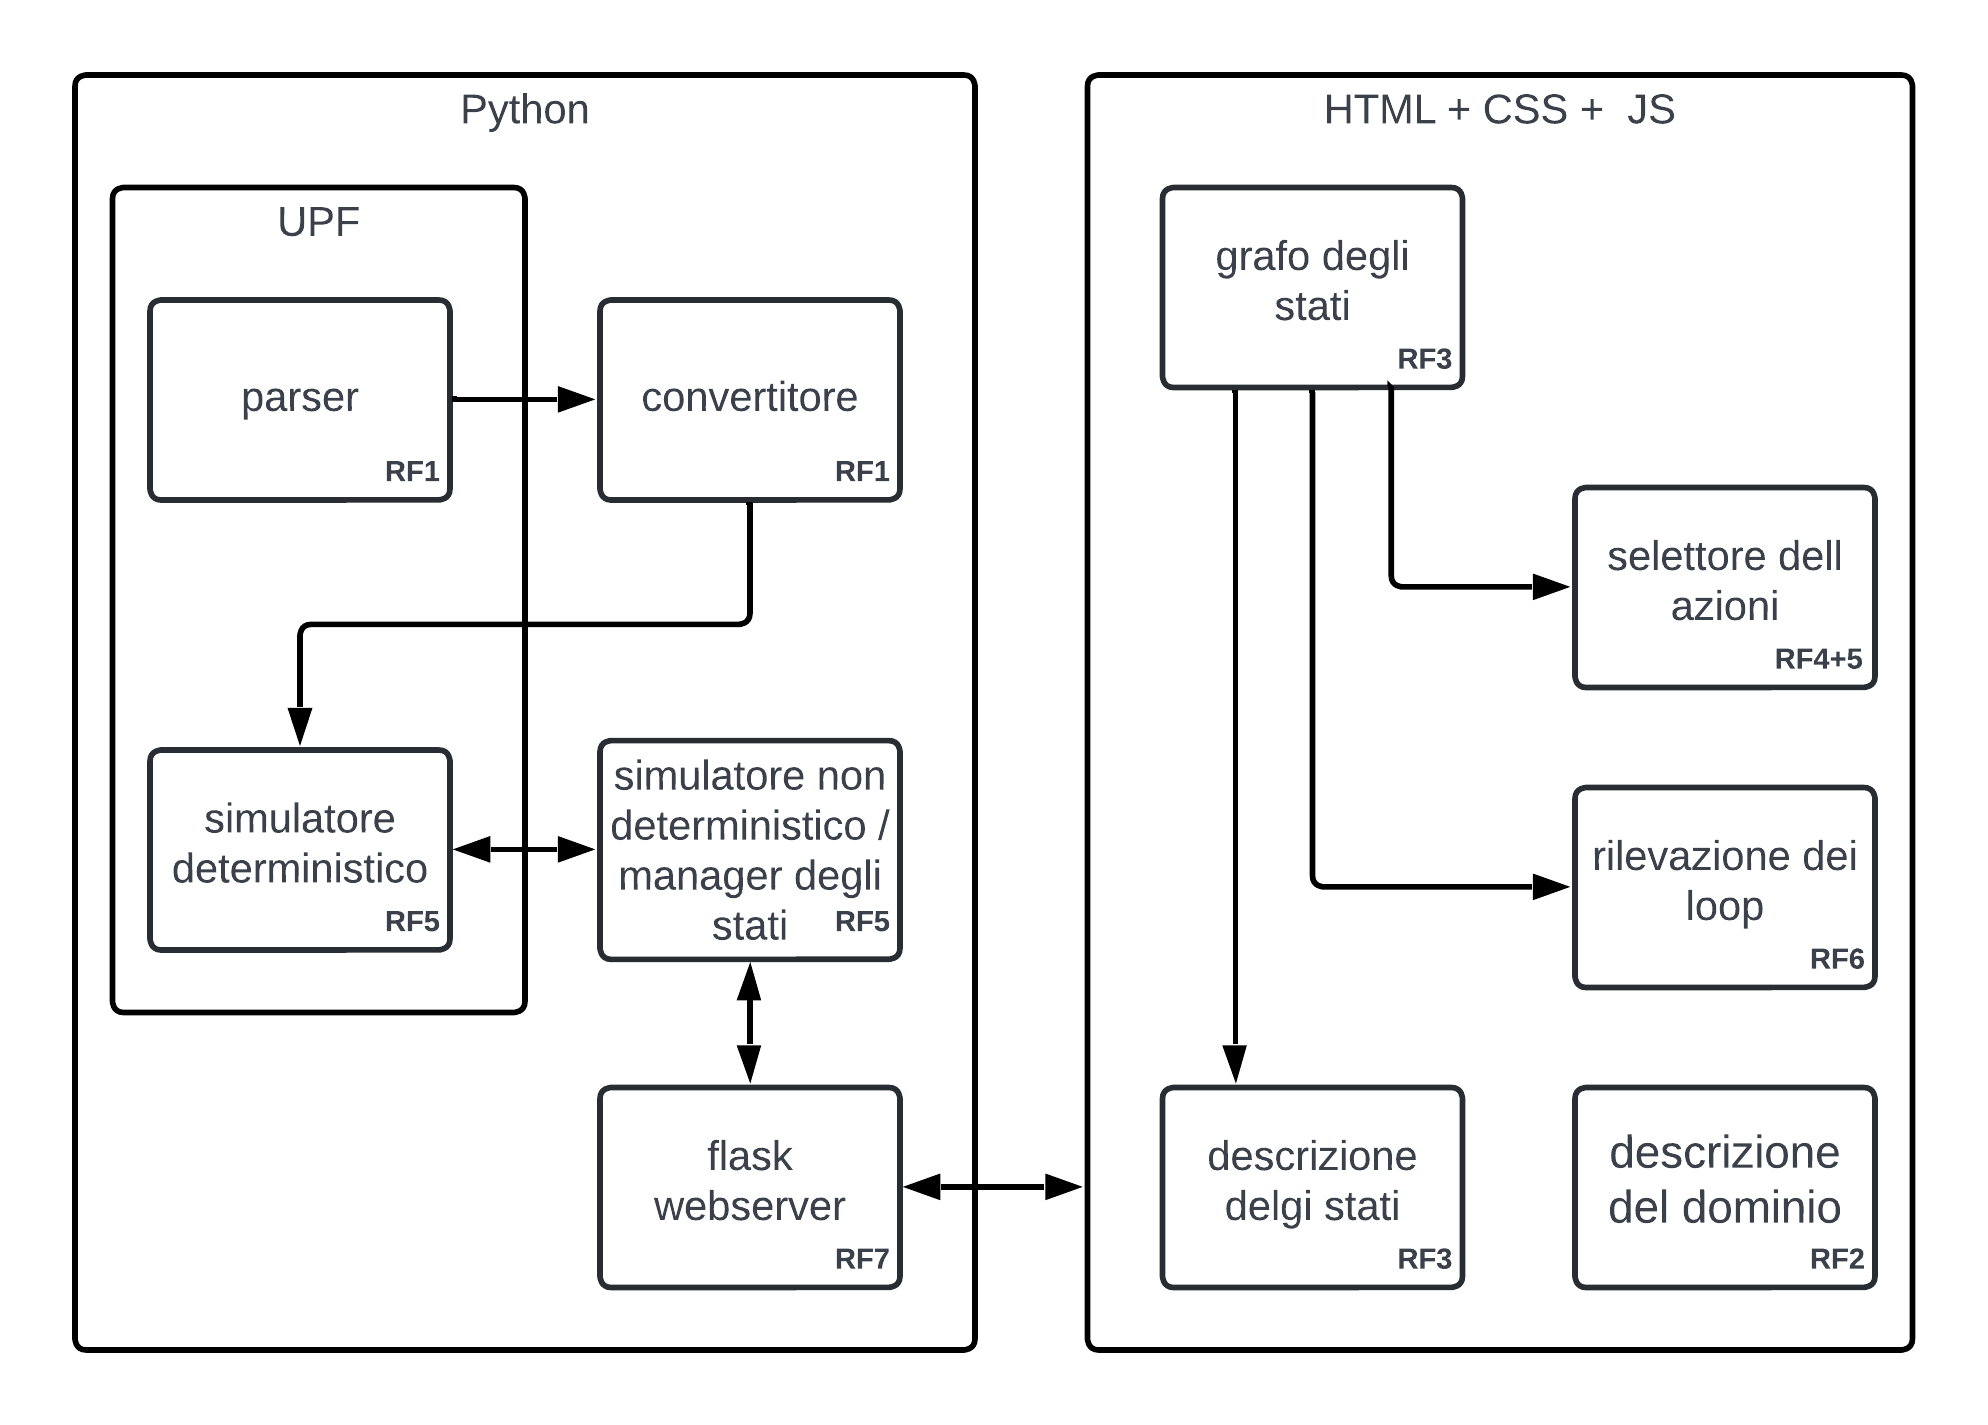
\includegraphics[width=1\linewidth]{figures/system_structure.png}
    \caption{\textit{I componenti principali del sistema}}
\end{figure}

Questa netta separazione tra il motore di simulazione e l'interfaccia utente è stata progettata per garantire una maggiore robustezza del sistema, assegnando in modo chiaro e distinto le responsabilità computazionali e quelle legate alla presentazione dei dati. Tale architettura modulare non solo facilita la manutenzione e l'estensibilità, ma permette anche un'elevata flessibilità nella gestione delle interfacce utente.

La comunicazione tra le due componenti avviene tramite chiamate API effettuate dalla GUI web, a cui il simulatore risponde con i dati elaborati. Questa struttura consente di mantenere il simulatore indipendente dall'interfaccia specifica, permettendo così l'integrazione di GUI di terze parti senza necessità di modifiche al nucleo computazionale del sistema.

\subsection{parser e convertitore}
Per motivi di efficienza la conversione descritta nella \textit{sez. \ref{sec:simulatore_non_deterministico}} viene applicata alle azioni durante la fase di parsing. Per fare questo ho modificato il parser presente nella libreria UPF. Vedi \textit{sez. \ref{sec:implementazione}} per maggiori informazioni.
L'output della fase di parsing è quindi un problema deterministico, in quanto ha già incorso la conversione.

\subsection{simulatore deterministico}
Il simulatore deterministico viene istanziato con il dominio convertito durante la fase di parsing e ha tre funzionalità.
\begin{itemize}
    \item \textit{Azioni Applicabili:} Dato uno stato del problema, il simulatore deterministico può produrre una lista di tutte le azioni che sono applicabili per quello stato.
    \item \textit{Esecuzione Azioni:} Dato uno stato e un'azione questo modulo può applicare l'azione allo stato per ottenere un nuovo stato, dove gli effetti dell'azione hanno preso atto
    \item \textit{Finalità degli Stati:} Dato uno stato  il simulatore può verificare qualora lo stato si tratti di uno stato finale per il problema oppure no.
\end{itemize}

\subsection{gestore degli stati}
\label{subsubsec: gestore_degli_stati}
Il gestore degli stati (GS) memorizza gli stati sotto forma di grafo orientato. Ogni nodo è associato ad un identificatore numerico univoco, uno stato della simulazione ed un'azione scelta per quello stato. Quest'ultimo campo è inizialmente nullo in quanto deve essere assegnato dall'utente. \\

Un'altra funzione del gestore degli stati è quella di fungere da wrapper per il simulatore deterministico. Più in dettaglio il GS implementa la traduzione tra simulatore deterministico e non deterministico descritta della \textit{sez. \ref{sec:simulatore_non_deterministico}}. \\
Dopo la conversione, le funzionalità esposte dal GS sono:
\begin{itemize}
    \item \textit{Azioni Applicabili:} Il GS produce una lista di azioni applicabili per uno stato della simulazione. Le azioni in questa lista sono poi raggruppate in base all'azione non deterministica da cui sono state generate.
    \item \textit{Esecuzione Azioni:} Dato uno stato e un'azione non deterministica $A$, il GS applica tutte le azioni deterministiche $A_n$ allo stato. I risultato delle azioni vengono poi usati per espandere il grafo. \\
\end{itemize}
Le restanti funzionalità del simulatore deterministico rimangono invariate. \\
Funzionalità uniche del GS sono:
\begin{itemize}
    \item {Rappresentazione del Grafo:} Il GS fornisce il grafo completo degli stati. (Vedi \textit{Formato del grafo})
    \item {Annullamento delle Azioni:} Il GS permette di annullare la scelta di un'azione per un determinato stato. Quest'azione comporta l'eliminazione di tutti gli stati che diventano irraggiungibili.
    \item {Rappresentazione di uno Stato:} Dato l'identificatore di uno stato il GS fornisce una rappresentazione dello stesso. (Vedi \textit{Formato dello stato})
\end{itemize}

\paragraph{Formato del grafo}
Il grafo è strutturato come una lista di nodi, ciascuno dei quali è caratterizzato dai seguenti parametri:

\begin{itemize}
    \item \textit{id:} Un identificatore numerico univoco che distingue ogni nodo all'interno del grafo.
    \item \textit{is\_final:} Un valore booleano che indica se lo stato associato al nodo è finale. Questo parametro è impostato a \texttt{true} se il nodo rappresenta uno stato finale.
    \item \textit{is\_loop:} Un valore booleano che indica se lo stato associato al nodo è l'inizio di un loop (vedi \textit{sez. \ref{rf6: rilevazione_loop}}).
    \item \textit{actions:} Una lista contenente le azioni che possono essere applicate allo stato associato al nodo.
    \item \textit{choice:} L'indice dell'azione selezionata dall'utente all'interno della lista \texttt{actions}. Questo campo può essere nullo se non è stata effettuata alcuna scelta dall'utente.
    \item \textit{diff:} Una lista che descrive le differenze tra lo stato $s$ rappresentato dal nodo corrente e lo stato $s'$ rappresentato dal nodo predecessore. Questa lista evidenzia le modifiche comportate dalla transizione dallo stato $s'$ allo stato $s$. Un nodo può avere più archi in entrata, pertanto il nodo predecessore è definito come il primo nodo che ha generato il nodo corrente.
    \item \textit{children:} Una lista degli identificatori (\texttt{id}) dei nodi che sono raggiungibili dal nodo corrente attraverso l'azione scelta. Questa lista rappresenta i possibili stati successivi nel grafo.
\end{itemize}

\subparagraph{Formato dello stato}
Uno stato è rappresentato come una lista di tutti i predicati e le risorse del problema, assieme ai valori che assumono nello stato in questione.

\subsection{flask webserver}
\label{subsec: webserver}
Il webserver ha due funzioni, entrambe legate alla presentazione della GUI all'utente. La prima è quella di servire dei file statici per la visualizzazione del sito. La seconda è quella di esporre degli endpoint che permettono la comunicazione tra il sito e il gestore degli stati.

Le API sono le seguenti:
\paragraph{get\_graph [GET]}
Questa API ritorna una vista completa del grafo in formato JSON.
\subparagraph{Esempio} La risposta dell'API per un grafo contenente due nodi
\begin{lstlisting}
{
  "nodes": [
    {
      "children": [1, 0],
      "choice": "pick-tower(b, a, c)",
      "diff": [],
      "id": 0,
      "is_final": false,
      "is_loop": false,
    },
    {
      "children": null,
      "choice": null,
      "diff": [
        "holding[a] := true", "emptyhand[] := false", 
        "on[a, c] := false", "clear[c] := true"
      ],
      "id": 1,
      "is_final": false,
      "is_loop": false,
    }
  ]
}
\end{lstlisting}

\paragraph{get\_fluents [GET]}
Fornisce un JSON contenente una lista di tutti i predicati e le risorse che descrivono il dominio del problema.
\subparagraph{Esempio} La risposta dell'API per il dominio \textit{blocksworld}. Solo un fluente è incluso per motivi di brevità.
\begin{lstlisting}
{
  "fluents": [
    {
      "name": "holding",
      "signature": [
        {
          "name": "b",
          "type": "block"
        }
      ],
      "str": "bool holding[b=block]",
      "type": "bool"
    },
  ]
}
\end{lstlisting}

\paragraph{get\_objects [GET]}
Fornisce un JSON contenente gli oggetti presenti nel problema suddivisi per tipo.
\subparagraph{Esempio} La risposta per un problema nel dominio \texttt{blocksworld}, contenente cinque blocchi.
\begin{lstlisting}
{
  "objects": {
    "block": [
      "a", "b", "c", "d", "e"
    ]
  }
}
\end{lstlisting}

\paragraph{state\_description?id [GET]}
L'API \texttt{state\_description} richiede un parametro numerico "id". Qualora questo parametro non sia fornito, o il valore non coincida con l'identificatore di un nodo nel grafo, un codice di errore sarà restituito. Rispettivamente \texttt{400} e \texttt{404}.
Nel caso di uso corretto della API viene ritornato un JSON contenente la descrizione dello stato indicato dal parametro "id".
Lo stato è descritto come una lista di predicati. Ad ogni predicato è associata una lista di parametri e il valore del predicato con quei parametri.
\subparagraph{Esempio} Il seguente esempio è lo stato iniziale del problema \texttt{jars} incluso nel casi di test.
\begin{lstlisting}
{
  "fluents": {
    "isjar": [
      {
        "parameters": [
          "jar2"
        ],
        "value": "false"
      },
      {
        "parameters": [
          "jar1"
        ],
        "value": "false"
      }
    ],
    "level": [
      {
        "parameters": [
          "jar2"
        ],
        "value": "0"
      },
      {
        "parameters": [
          "jar1"
        ],
        "value": "2"
      }
    ]
  }
}
\end{lstlisting}


\paragraph{get\_aviable?id [GET]}
L'API \texttt{get\_aviable} richiede un parametro numerico "id". Qualora questo parametro non sia fornito, o il valore non coincida con l'identificatore di un nodo nel grafo, un codice di errore sarà restituito. Rispettivamente \texttt{400} e \texttt{404}.
Nel caso di uso corretto della API viene ritornato un JSON contenente una descrizione delle azioni applicabili allo stato indicato.
Le azioni sono descritte dal loro nome, i parametri effettivi e una lista di possibili effetti.
\subparagraph{Esempio}
Questo è la descrizione delle azioni applicabili allo stato iniziale del problema \texttt{jars}. Solo una azione è inclusa per motivi di brevità.
\begin{lstlisting}
{
  "actions": [
    {
      "args": [ "jar1", "jar2" ],
      "effects": [
        [
          "level(from) -= 1",
          "level(to) += 1"
        ]
      ],
      "name": "pour"
    },
    ...
  ]
}
\end{lstlisting}

\paragraph{choose?id\&n [POST]}
Questa API prende in input due parametri di tipo numerico:
\begin{itemize}
    \item id: L'identificatore dello stato a cui si vuole applicare un'azione.
    \item n: L'indice dell'azione da applicare all'interno del vettore fornito dalla API \texttt{get\_aviable}
\end{itemize}
In caso uno o più dei valori non sia fornito l'API restituisce un codice d'errore \texttt{400}. \\
In caso l'id non corrisponda ad alcuno stato si otterrà un codice d'errore \texttt{404}. \\
In caso "n" sia negativo o maggiore del numero di azioni possibili per lo stato, si otterrà il codice di errore \texttt{404}. \\
In caso di esecuzione corretta dell'API, l'azione indicata sarà applicata allo stato. Questa azione aggiorna il grafo e ritorna il codice \texttt{200}.

\paragraph{undo\_choice?id [POST]}
L'API \texttt{undo\_choice} richiede un parametro numerico "id". Qualora questo parametro non sia fornito, o il valore non coincida con l'identificatore di un nodo nel grafo, un codice di errore sarà restituito. Rispettivamente \texttt{400} e \texttt{404}.
Nel caso  di uso corretto della API il simulatore annulla l'azione scelta per lo stato indicato dal parametro "id". Tutti gli stati resi irraggiungibili da questa modifica saranno eliminati.

\subsection{Interfaccia Grafica Utente}
L'interfaccia grafica del simulatore viene presentata all'utente sotto forma di sito web. Questo sito è servito localmente dal server presente nel applicazione e descritto nella \textit{sez. \ref{subsec: webserver}}.
Il sito è composto di una sola pagina divisa a sua volta in tre sezioni, come mostrato in \textit{fig. \ref{fig:screenshot}}. Queste sono: il visualizzatore del grafo, il descrittore degli stati e il descrittore del problema e del dominio.
\begin{figure}
    \centering
    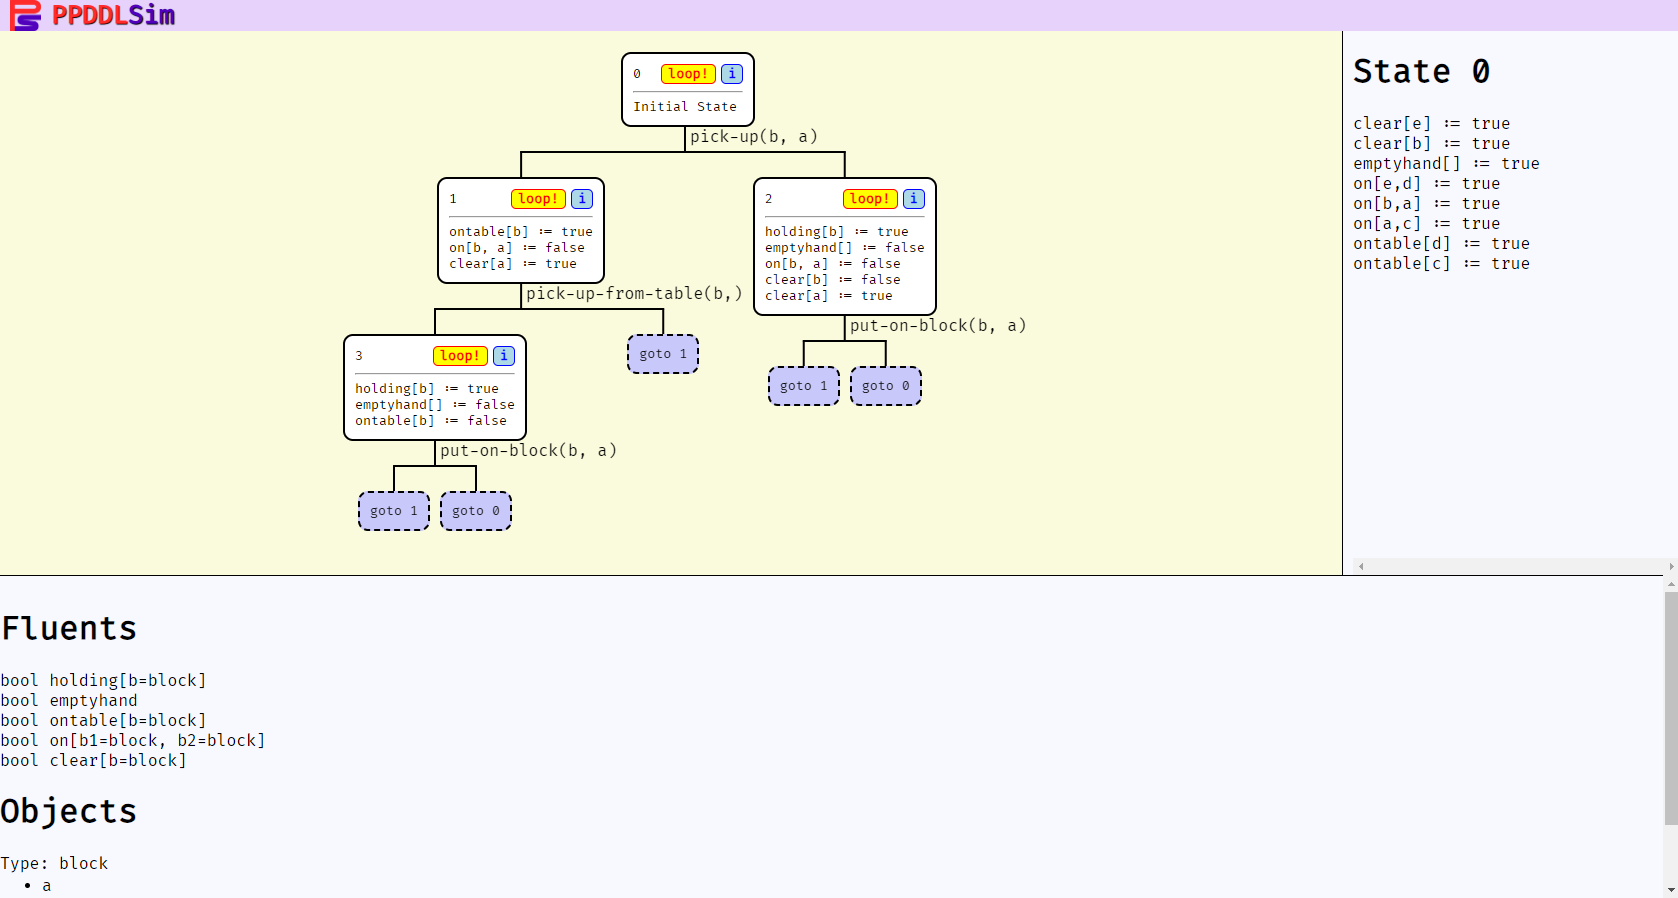
\includegraphics[width=1\linewidth]{figures/PPDDLSim_screenshot_loop.png}
    \caption{\textit{Una schermata dell'interfaccia utente}}
    \label{fig:screenshot}
\end{figure}
\begin{figure}
    \centering
    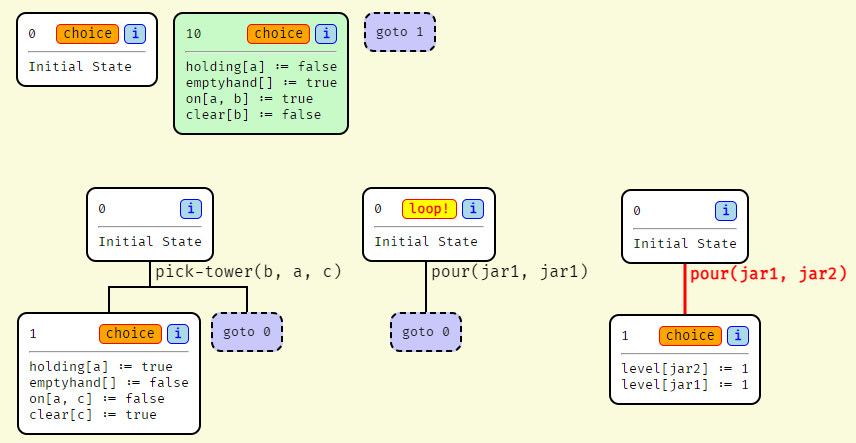
\includegraphics[width=1\linewidth]{figures/cards.png}
    \caption{\textit{I diversi tipi di nodo nel visualizzatore}}
    \label{fig:nodi}
\end{figure}
\begin{figure}
    \centering
    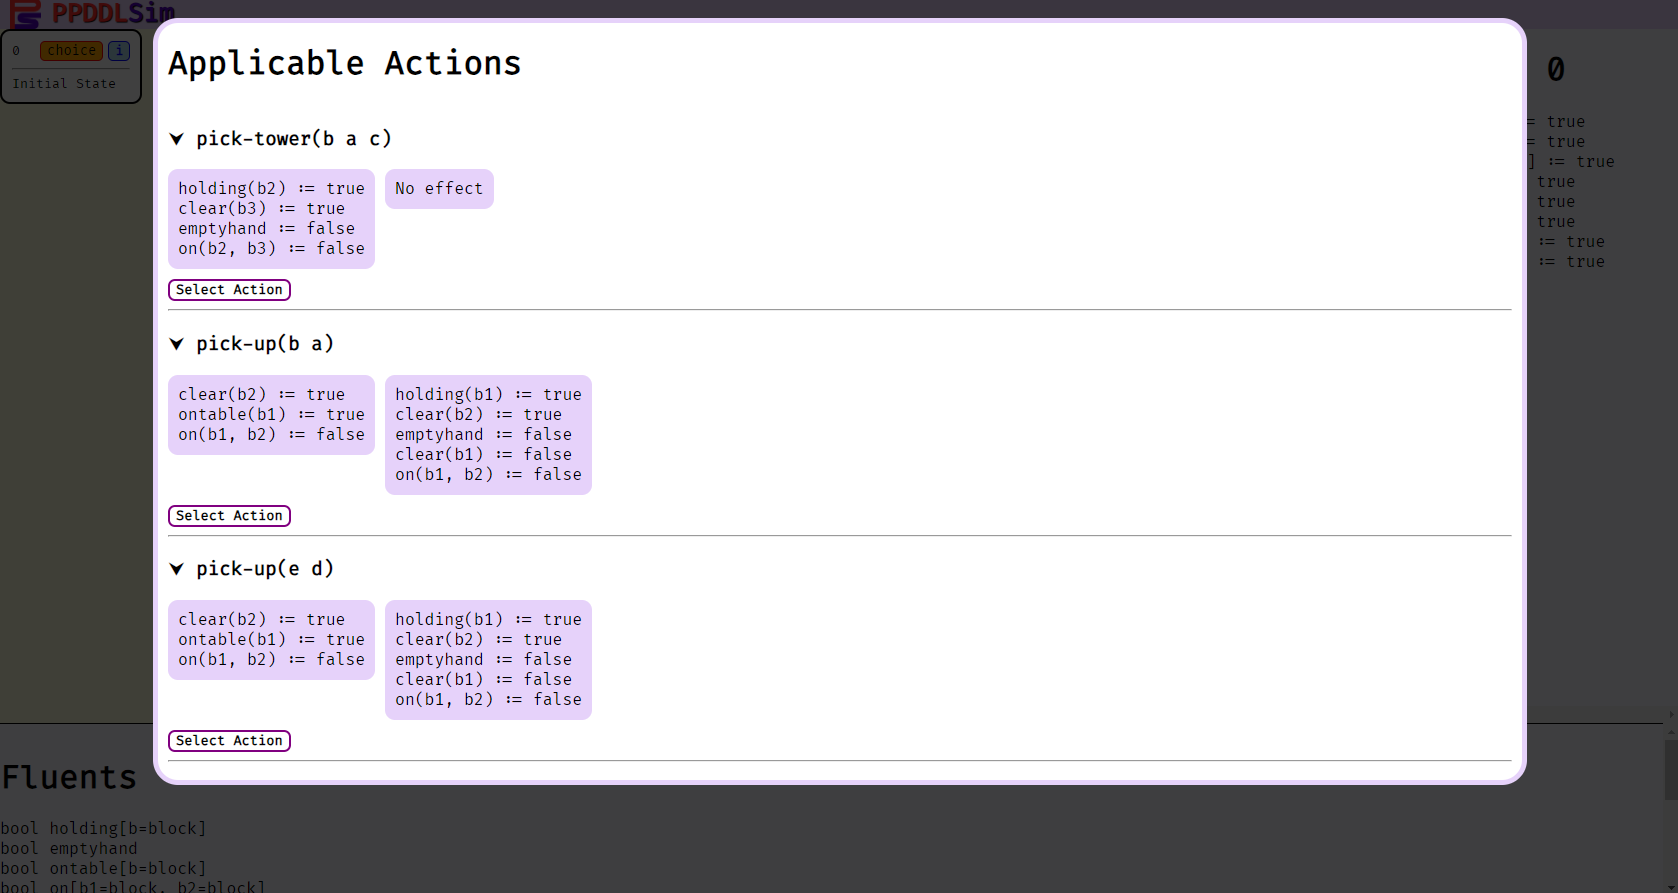
\includegraphics[width=1\linewidth]{figures/applicable_actions_screen.png}
    \caption{\textit{La schermata di selezione delle azioni}}
    \label{fig:selezione_azioni}
\end{figure}
\paragraph{Vista Del Grafo}
La vista del grafo presenta tutti gli stati esplorati nella simulazione. Gli stati, o nodi, sono rappresentati da rettangoli come mostrato in \textit{fig. \ref{fig:nodi}}. \\
Ogni nodo ha un identificatore e una lista delle differenze dallo stato precedente, eccetto lo stato iniziale in quanto esso non ha stati precedenti. Il bottone blu mostra una descrizione dello stato o la nasconde in caso sia già aperta. \\
Gli stati in cui non è stata ancora fatta alcuna scelta presentano un bottone "choice", che mostra all'utente la schermata di scelta delle azioni (\textit{fig. \ref{fig:selezione_azioni}}). \\
Le transizioni tra uno stato e i successivi sono rappresentate da una linea nera, il nome e i parametri dell'azione. \\
Muovere il mouse sulla linea la rende rossa, e premerla permette all'utente di annullare l'azione. \\
Gli stati iniziali di un loop sono contrassegnati da un indicatore con la scritta "loop!" rosso su giallo.

Per rendere il grafo più leggibile non sono mostrati gli archi che conducono a uno stato precedentemente visitato. Sono invece sostituiti da un nodo tratteggiato su sfondo viola.

\paragraph{Descrittore Degli Stati}
Il descrittore degli stati viene aperto cliccando il tasto blu su uno degli stati nella vista del grafo. Compare sulla destra del grafo come mostrato in \textit{fig. \ref{fig:screenshot}}.\\
La descrizione comprende l'identificatore numerico dello stato e una lista di tutti i predicati e i loro valori. I predicati con valore \texttt{false} sono omessi per leggibilità. \\
La sezione può essere liberamente allargata o ristretta.

\paragraph{Descrittore Di Dominio E Problema}
La sezione inferiore della pagina contiene una descrizione dal problema e del dominio. Questo include una lista degli oggetti presenti nel problema ordinati per tipo e una lista di predicati. \\
Questa sezione della pagina può essere ingrandita o resa più piccola trascinandone il limite superiore in alto o in basso.

\section{Implementazione}
\label{sec:implementazione}
Nella seguente sezione descriverò le tecniche implementative e i paradigmi utilizzati per la costruzione del simulatore. Questo includerà una descrizione più dettagliata dei componenti indicati in \textit{sez. \ref{sec: architettura}}, estratti del codice e considerazioni riguardo possibili futuri miglioramenti.

\subsection{Panoramica del funzionamento del simulatore}
Il simulatore può essere eseguito tramite il comando \texttt{py main.py domain.pddl problem.pddl}, dove \texttt{domain.pddl} e \texttt{problem.pddl} rappresentano rispettivamente i percorsi del file di dominio e il file del problema in formato PDDL.
Una volta avviato, il programma legge i file indicati da linea di comando. Qualora i file non vengano trovati nel sistema o non vengano riconosciuti come file PDDL validi, un errore sarà mostrato a linea di comando. \\
In caso di avvio corretto del programma, invece, un link web alla GUI verrà mostrato al utente. Il link verrà inoltre aperto automaticamente con il browser predefinito di sistema. \\
A seguito dell'avvio corretto dell'applicazione il terminale mostra soltanto informazioni di debug, mentre l'interazione con l'utente è svolta interamente dalla GUI web.

\subsection{argparse} Il programma utilizza la libreria standard python \texttt{argparse} per gestire i parametri di input. Questo approccio rende la gestione dei parametri robusta e flessibile, garantendo interoperabilità tra differenti terminali e sistemi operativi. \\
Oltre ai parametri posizionali \texttt{dominio} e \texttt{problema} il comando accetta le flag \texttt{-h} e \texttt{-s}. \texttt{-h} presenta una schermata di aiuto all'utente in linea di comando, mentre \texttt{-s} impedisce al programma di aprire il browser per mostrare l'interfaccia grafica.

\subsection{Parsing} Per il parsing dei file ho modificato la classe \texttt{PDDLReader} della libreria unified-planning (UPF), aggiungendo supporto per le feature non deterministiche di PPDDL. Questo approccio è più stabile rispetto all'implementazione di un intero parser, in quanto si basa sul lavoro già svolto da molteplici collaboratori alla libreria open source UPF. Ampliare le funzionalità della libreria mi ha permesso di integrare il resto della mia applicazione con molti degli strumenti offerti da UPD. Questo include una classe per la rappresentazione di un problema e il simulatore sequenziale.

La classe UPD che gestisce la lettura del file è \texttt{PDDLReader}. Più in particolare il suo metodo \texttt{parse\_problem} che prende in input il percorso di un dominio, un problema, e restituisce un oggetto della classe \texttt{Problem} che rappresenta il problema. Questa è la classe che ho modificato per supportare il non determinismo.
Il file viene letto tramite \texttt{pyparsing} e ne viene derivata una struttura ad albero. Questo albero viene poi usato per la costruzione dell'oggetto \texttt{Problem}. \\
Il mio approccio si basa sull'aggiungere un passaggio extra che modifica l'albero di parsing prima di proseguire con la normale elaborazione del file. \\
La conversione del file influenza solo le azioni del dominio, quindi andrò a trattare solo quelle. Il campo "name" per le azioni è obbligatorio mentre "eff" (effetto) è opzionale. Il nome è rappresentato come una stringa e l'effetto è rappresentato da una espressione annidata, che può essere vista a sua volta come un albero. Più in particolare l'espressione annidata è un vettore dove ogni elemento può essere un token (di tipo stringa) o un'altra espressione annidata.

La conversione delle azioni, come illustrata in \textit{sez. \ref{sec:simulatore_non_deterministico}} involve la "scomposizione" di tutte le azioni che contengono più possibili effetti. La parte più complessa di questa procedura è determinare il set dei possibili effetti di un'azione non deterministica. L'algoritmo che ho utilizzato per effettuare la conversione è il seguente:

\RestyleAlgo{ruled}
\begin{algorithm}
\caption{Conversione Delle Azioni}\label{alg:convert}
\KwData{azioniNonDeterministiche}
\KwResult{azioniDeterministiche}
$azioniDeterministiche \gets []$\;
\While{$\|azioniNonDeterministiche\|>0$}{
    $azione \gets azioniNonDeterministiche.pop()$\;
    \uIf{\Not azione.hasEffect()}{
        $azioniDeterministiche.push(azione)$\;
        \Continue \Comment*[l]{azioni senza effetti sono deterministiche}
    }
    
    $opzioni \gets trovaOpzioni(azione)$\;
    \uIf{$\|opzioni\|== 0$}{
        $azioniDeterministiche.push(azione)$\;
        \Continue \Comment*[l]{azioni senza opzioni varie sono deterministiche}
    }
    $i \gets 0$\;
    \ForEach {$o\in opzioni$}{
        $nuovaAzione \gets copy(azione)$\;
        $nuovaAzione.nome \gets azione.nome + "\_deff" + i$\;
        $converti(nuovaAzione,\ o)$\;
        $azioniNonDeterministiche.push(nuovaAzione)$\;
        $i++$\;
    }
}
\end{algorithm}
Se un'azione è deterministica viene spostata alla lista di azioni deterministiche senza apportare modifiche. Questo è il caso base a cui verranno portate anche le azioni non deterministiche.
La funzione \texttt{trovaOpzioni}, illustrata più avanti, esegue una visita in ampiezza dell'effetto dell'azione e si ferma al primo \texttt{oneof} trovato. Le opzioni che ritorna sono i possibile outcome del \texttt{oneof}. \\
Vengono create $\|opzioni\|$ nuove azioni, e in ognuna il primo \texttt{oneof} viene sostituito con una delle opzioni. \\
Le nuove azioni vengono aggiunte alla lista di azioni potenzialmente non deterministiche in quanto potrebbero contenere altre clausole \texttt{oneof}. In caso non ne contengano saranno spostane nella lista di azioni deterministiche nel cicli seguenti.

La visita in ampiezza accennata sopra segue delle regole specifiche:
\begin{itemize}
    \item Se l'espressione non è una formula atomica il primo valore è l'operatore.
    \item Se l'operatore è "\texttt{and}": tutti valori successivi vanno aggiunti alla visita, data la forma $(and\ e_1\ e_2\ \dots\ e_n)$.
    \item Se l'operatore è "\texttt{when}" o "\texttt{forall}": solo il terzo valore viene aggiunto alla visita in quanto non serve cercare \texttt{oneof} nella condizione o lo lista di variabili. \\ 
    $([when|forall]\ [condition|variables]\ effect)$
    \item Se l'operatore è "\texttt{oneof}": tutti i valori successivi sono le possibili opzioni. $(oneof\ o_1\ o_2\ \dots\ o_n)$
\end{itemize}
Altri operatori come "\texttt{not}" e "\texttt{change}" non possono avere effetti come argomenti successivi, quindi non vengono considerati nella conversione.

\begin{algorithm}
\caption{Individuazione delle opzioni del primo oneof con visita in ampiezza}\label{alg:findOneof}
\SetKwFunction{TrovaOpzioni}{trovaOpzioni}
\SetKwProg{Fn}{Function}{:}{}
\Fn{\TrovaOpzioni{azione}}{
    oneofTrovato = False\;
    opzioni=[]\;
    codaVisita = [azione.effect[0]]\;
    \While{\Not oneofTrovato \And $\|codaVisita\| > 0$}{
        corrente = codaVisita.pop()\;
        operatore = corrente[0]\;
        \uIf{operatore=="and"}{
            \For{i=1 \KwTo $\|corrente\|$} {
                codaVisita.push(corrente[i])\;
            }
        }
        \uElseIf{operatore=="when" \Or operatore=="forall"}{
            codaVisita.push(corrente[2])\;
        }
        \ElseIf{operatore=="oneof"}{
            oneofTrovato = True\;
            \For{i=1 \KwTo $\|corrente\|$}{
                opzioni.push(corrente[i])\;
            }
        }
    }
    \Return opzioni\;
}
\end{algorithm}

La funzione "\texttt{converti}" segue una logica simile a "\texttt{trovaOpzioni}". \\
Data un'azione e un effetto (chiamato opzione in questo caso) la funzione esegue una visita dell'effetto dell'azione con le stesse regole indicate sopra. Una volta individuato il primo \texttt{oneof}, esso viene sostituito con l'effetto indicato. Lo pseudocodice per la conversione è indicato in \textit{Algorithm 3}.

\begin{algorithm}
\caption{Sostituisci il primo oneof dell'azione con l'opzione indicata}\label{alg:Converti}
\SetKwFunction{Converti}{converti}
\SetKwProg{Fn}{Function}{:}{}
\Fn{\Converti{azione, opzione}}{
    modificato = False\;
    codaVisita = [azione.effect[0]]\;
    \While {$\|codaVisita\| > 0$ \And \Not modificato}{
        corrente = codaVisita.pop()\;
        operatpre = corrente[0]\;
        \uIf {operatore == "and"}{
            j = 1\;
            \While {$j < \|corrente\|$ \And \Not modificato}{
                \uIf {corrente[j][0] == "oneof"}{
                    corrente[j] = opzione\;
                    modificato = True\;
                }
                \uElse{
                    codaVisita.push(corrente[j])\;
                }
                j++\;
            }
        }
        \uElseIf{op == "when" \Or operatore=="forall"}{
            \uIf {corrente[2][0] == "oneof"}{
                corrente[2] = opzione\;
                modificato = True\;
            }
            \uElse{
                codaVisita.push(corrente[2])\;
            }
        }
    }
}
\end{algorithm}
La lista di azioni deterministiche viene poi utilizzata all'interno della classe \texttt{PDDLReader} per costruire il problema.

La fork della libreria appropriatamente modificata è disponibile al pubblico presso la repository "\texttt{https://github.com/diego-oniarti/unified-planning}".

\paragraph{Considerazioni sulla complessità temporale}
L'algoritmo illustrato nello pseudocodice non è ottimale dal punto di vista temporale, in quanto una visita dell'albero viene effettuata sia in \texttt{trovaOpzioni} che in \texttt{converti} per individuare la stessa clausola \texttt{oneof} nell'effetto. \\
Un altro problema sorge in \textit{Algorithm \ref{alg:convert}}. L'algoritmo proposto può effettuare la conversione di una clausola \texttt{oneof} più volte in caso sia situata in una clausola \texttt{and} assieme ad altri \texttt{oneof}. Questo problema potrebbe essere risolto con tecniche di programmazione dinamica.

\subsection{Gestore Degli Stati}
Il gestore degli stati illustrato nella \textit{sez. \ref{subsubsec: gestore_degli_stati}} è implementato come una classe \texttt{NonDeterministicSimulator} che funge da wrapper per la classe \texttt{SequentialSimulator} di \texttt{unified-planning}. \\
Il \texttt{NonDeterministicSimulator} (NDS) contiene un'istanza di un simulatore sequenziale ed una mappa $id\to nodo$ che rappresenta il grafo degli stati. Ogni nodo viene usato per memorizzare uno stato della simulazione. \\
Quando un nodo viene creato vengono anche calcolate le possibili azioni che possono essere eseguite nello stato corrispondente. Una lista contenente queste azioni è salvata nel nodo, evitando di doverla calcolare più volte. Lo stesso vale per le differenze tra lo stato corrente e quello precedente. \\
Il \texttt{NonDeterministicSimulator} svolge la rilevazione dei loop indicata nella \textit{sez. \ref{rf6: rilevazione_loop}}. Questo processo viene svolto ogni volta che viene alterato il grafo. Il processo è illustrato in \textit{Algorithm 4}.

\begin{algorithm}
\caption{Rilevazione dei loop nel grafo degli stati}\label{alg:loop}
\KwData{G \Comment{Il grafo degli stati}}
$G'\gets trasponi(G)$\Comment*[r]{Calcola il grafo trasposto}
\For{$n \in G.nodi$}{
    $D\gets BFS(G,\ n)$\Comment*[l]{set di nodi raggiungibili in $G$ partendo da $n$}
    $D'\gets BFS(G',\ n)$\;
    \If{$D=D'$}{
        $n.loop \gets true$
    }
}
\end{algorithm}

\subsection{Visualizzatore del grafo}
La sezione principale dell'interfaccia web (\textit{fig. \ref{fig:screenshot}}) è il visualizzatore interattivo del grafo degli stati. Il visualizzatore richiede l'intero grafo tramite l'API \texttt{get\_graph} durante il caricamento della pagina e ogni volta che viene apporta una modifica allo stato del simulatore. \\
Per motivi di leggibilità il grafo viene visualizzato come un albero. Questo è fatto grazie all'aggiunta di nodi fittizi chiamati "$goto_n$".
Questa conversione da grafo ad albero è svolta mediante l'\textit{Algorithm 5}. \\
\begin{algorithm}
\caption{Aggiunta dei nodi $goto_n$}\label{alg:aggiunta_goto}
\KwData{G \Comment{Il grafo originale degli stati}}
\KwResult{T \Comment{L'albero ottenuto dalla conversione}}
$Q \gets emptyQueue()$\;
$Q.push(G.start)$\Comment{La visita inizia del nodo legato allo stato iniziale del problema}
$head \gets newNode(G.start)$\;
$V \gets emptySet()$\Comment{set dei nodi visitati}
\While{$\|Q\|>0$}{
    $c \gets Q.pop()$\;
    $V.add(c)$\;
    \For{$o \in o.outgoing$}{
        \uIf{V.has(o)}{
            $c.addChild(newGoto(o.id))$\;
        }\Else{
            $c.addChild(newNode(o))$\;
            $V.add(o)$\;
            $Q.push(o)$\;
        }
    }
}
\end{algorithm}
L'algoritmo si basa su una visita in ampiezza del grafo a partire dallo stato iniziale. Quando si incontra una transizione verso un nodo già visitato $n$ la si sostituisce con una visita verso un nuovo nodo $goto_n$. \\
I nodi $goto_n$ quindi indicano all'utente che un'azione riconduce il simulatore ad uno stato $n$ già visitato.

\subsection{Elementi HTML e Canvas}
I nodi e i nomi delle azioni scelte (\textit{fig. \ref{fig:nodi}}) sono mostrati tramite elementi HTML mentre le linee che indicano le transizioni sono disegnate su una Canvas come combinazione di primitive. \\
Delegare il rendering degli elementi con testo al browser offre diversi vantaggi rispetto all'opzione alternativa di disegnare l'intero grafo sulla canvas:
\begin{itemize}
    \item \textit{Interazione:} Il testo può essere facilmente selezionato e copiato.
    \item \textit{Accessibilità:} La dimensione del testo è affetta dallo zoom della pagina e il testo può essere letto da motori di Text-To-Speech. Questo agevola l'interazione con l'interfaccia da parte di utenti ipovedenti. 
\end{itemize}
Le linee sono disegnate sulla canvas per mantenere al minimo la quantità di elementi HTML aggiunti dinamicamente alla pagina, migliorando così le prestazioni del sito.

Il posizionamento dei nodi è calcolato in maniera che non siano possibili sovrapposizioni tra elementi tramite il procedimento ricorsivo illustrato in \textit{Algorithm 6}. L'algoritmo costruisce per ogni nodo $n$ un rettangolo che contiene l'intero albero avente $n$ come radice. Questo rettangolo è caratterizzato dalle proprietà \texttt{width}, \texttt{height} e dal vettore \texttt{pos}. Esse rappresentano la posizione dell'angolo superiore sinistro del rettangolo, la sua altezza e larghezza.\\
\begin{algorithm}
\caption{Posizionamento dei nodi}\label{alg:calc_size}
\KwData{G \Comment{L'albero degli stati}}
$cs \gets 10$ \Comment*[l]{Lo spazio tra i figli di un nodo}
$ls \gets 20$ \Comment*[l]{Lo spazio tra un nodo e i figli}
istanzia un elemento HTML $n.elem$ per ogni nodo $n$ in G\;
\SetKwFunction{Position}{posiziona}
\SetKwProg{Fn}{Function}{:}{}
\Fn{\Position{n}}{
    $n.position \gets (0,0)$\;
    \If{$\|n.children\|==0$}{
        \Comment{Se il nodo è una foglia prende le dimensioni dell'elemento HTML}
        $n.width \gets n.elem.width$\;
        $n.height \gets n.elem.height$\;
        \Return\;
    }
    $childrenWidth \gets max(0,\ cs(\|c.children\|-1))$\;
    $maxChildHeight \gets 0$\;
    \For {$c\in n.children$} {
        $posiziona(c)$\;
        $childrenWidth += c.width$\;
        $maxChildHeight \gets max(maxChildHeight, c.height)$\;
    }
    $n.width \gets max(c.elem.width,\ childrenWidth)$\;
    $n.height \gets c.elem.height + maxChildHeight + ls$\;
    $n.elem.x \gets \frac{n.width-n.elem.width}{2}$\;
    $x\gets -\frac{n.width}{2}$\;
    \For {$c \in n.children$} {
        $c.position.x \gets x$\;
        $c.position.y \gets n.elem.height+ls$\;
        $x += c.width+cs$\;
    }
}
posiziona(G.head)\;
\end{algorithm}
Il diagramma mostrato in \textit{fig. 5} illustra più chiaramente il ruolo delle proprietà usate per il posizionamento dei nodi. \\
\begin{figure}
    \centering
    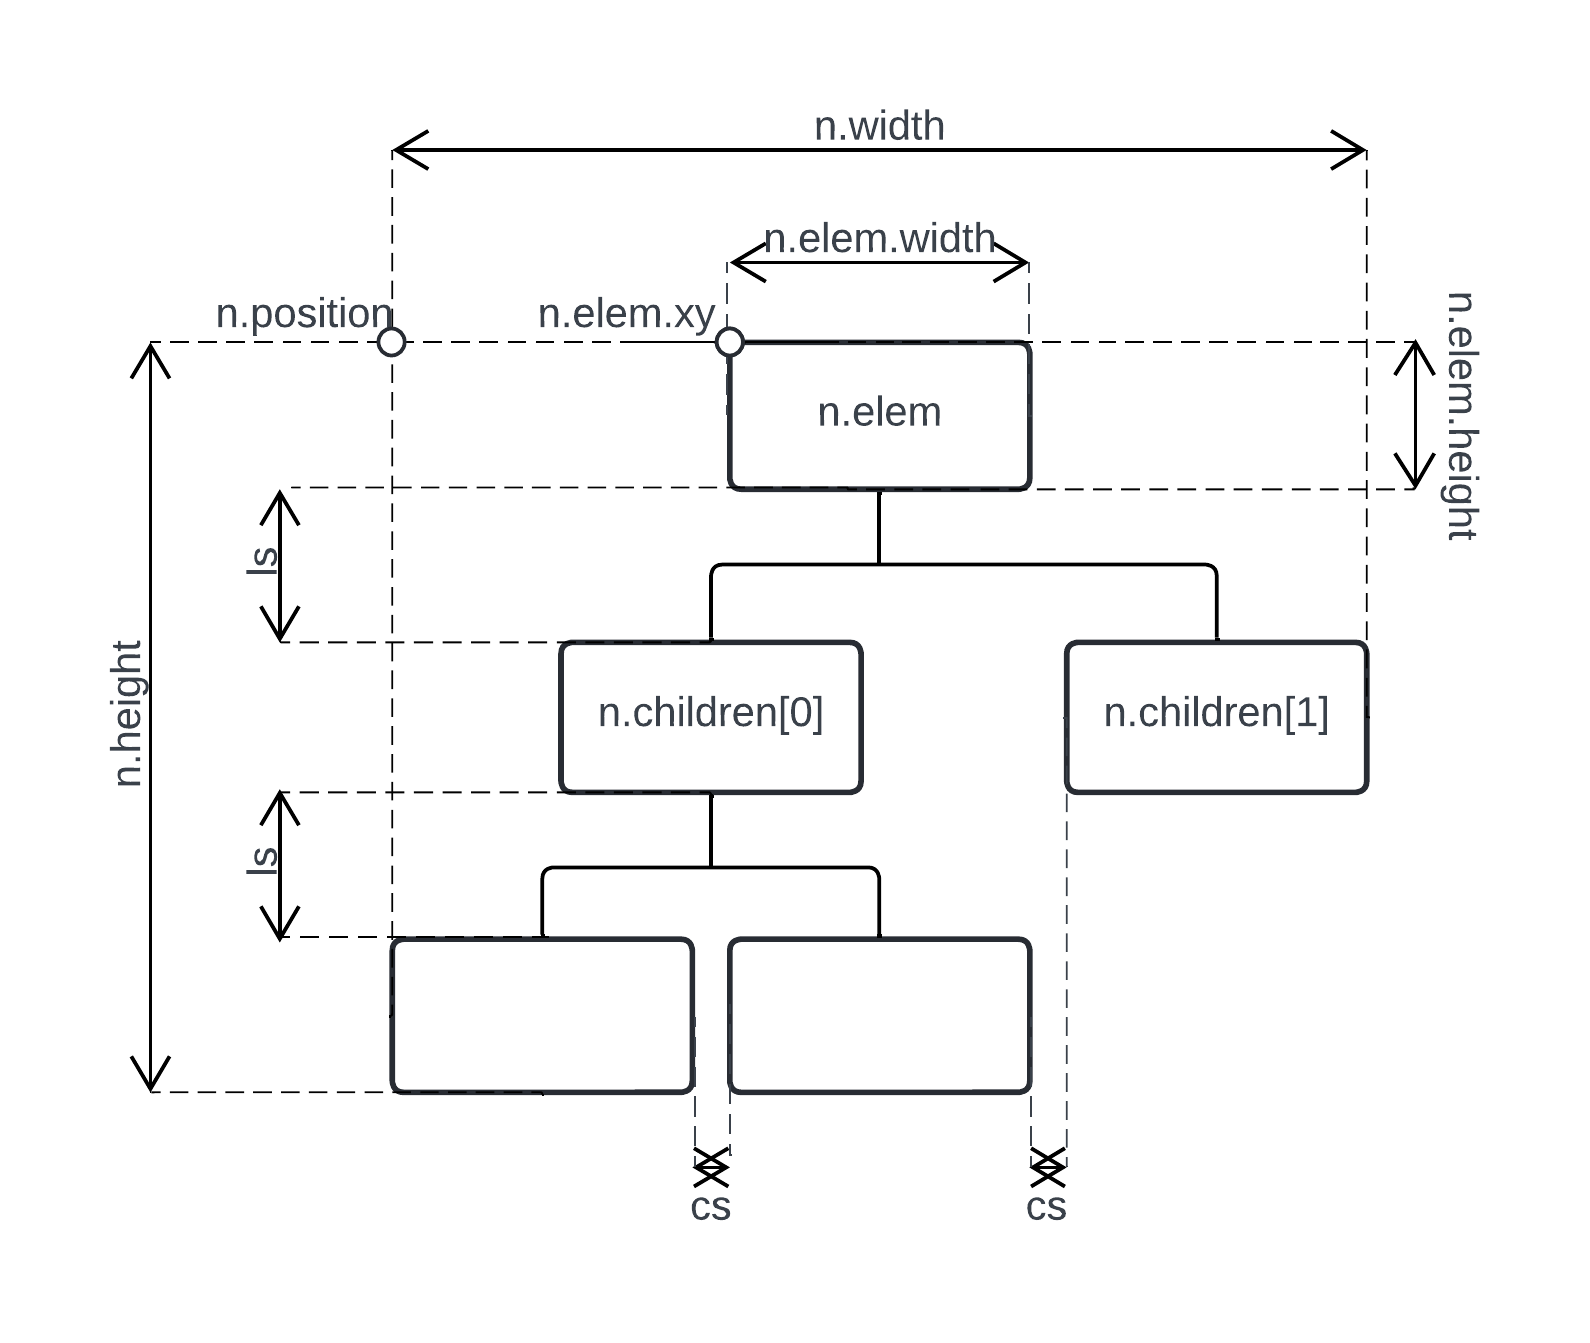
\includegraphics[width=0.5\linewidth]{figures/sizing.png}
    \caption{\textit{I parametri usati per il posizionamento di 5 nodi}}
\end{figure}

\subsection {Spostamento Dell'Albero}
L'albero può essere mosso trascinando il mouse all'interno del visualizzatore. Questo effetto è realizzato misurando la direzione in cui viene trascinato il mouse e applicando lo stesso spostamento ad ognuno dei nodi. \\
Se l'intero albero viene trascinato al di fuori dell'area del visualizzatore all'utente sarà presentato un bottone con la scritta "Center View". Premere questo bottone posiziona l'albero nell'angolo superiore sinistro della finestra.

\chapter{Validazione}
Ho svolto la validazione del progetto utilizzando diverse tecniche per ogni componente. 
\begin{itemize}
    \item Le API sono state testate mediante l'utilizzo di \textit{Postman}\cite{postman} per assicurarmi della correttezza sia del contenuto che del formato delle risposte.
    \item I metodi più complessi delle classi python sono stati soggetti a test unitari mediante la libreria \textit{pytest}.
    \item Ogni funzione dell'interfaccia web è stata testata manualmente seguendo le varie azioni che un utente potrebbe compiere.
    \item L'intero progetto è stato testato su diversi domini presi dalle traccie non deterministiche del concorso IPC e prodotti su misura.
\end{itemize}

\section{Esempio:}
Nel seguente esempio mostrerò un caso di test. Questo comprende: un dominio non deterministico "blocksworld", un problema associato a questo dominio, un'intuizione del dominio e del problema, e una soluzione al problema ottenuta tramite il simulatore.
Il dominio "blocks-domain" modella un mondo composto da dei blocchi e un tavolo. I blocchi possono essere presi o posati, sia sul tavolo che su altri blocchi. Quando un blocco viene preso c'è la possibilità che esso possa cadere sul tavolo, modellando la possibile imprecisione del braccio che muove i blocchi.
\paragraph{Dominio}
Il dominio è il seguente:
\begin{lstlisting}
(define (domain blocks-domain)
  (:requirements :non-deterministic :equality :typing)
  (:types block)
  (:predicates (holding ?b - block) (emptyhand) 
    (ontable ?b - block) (on ?b1 ?b2 - block) (clear ?b - block))
  (:action pick-up
    :parameters (?b1 ?b2 - block)
    :precondition (and (not (= ?b1 ?b2)) (emptyhand)
      (clear ?b1) (on ?b1 ?b2))
    :effect
      (oneof
        (and (holding ?b1) (clear ?b2) (not (emptyhand))
          (not (clear ?b1)) (not (on ?b1 ?b2)))
        (and (clear ?b2) (ontable ?b1) (not (on ?b1 ?b2))))
  )
  (:action pick-up-from-table
    :parameters (?b - block)
    :precondition (and (emptyhand) (clear ?b) (ontable ?b))
    :effect (oneof (and) (and (holding ?b) (not (emptyhand))
        (not (ontable ?b))))
  )
  (:action put-on-block
    :parameters (?b1 ?b2 - block)
    :precondition (and (holding ?b1) (clear ?b2))
    :effect (oneof (and (on ?b1 ?b2) (emptyhand) (clear ?b1)
        (not (holding ?b1)) (not (clear ?b2)))
      (and (ontable ?b1) (emptyhand) (clear ?b1)
        (not (holding ?b1))))
  )
  (:action put-down
    :parameters (?b - block)
    :precondition (holding ?b)
    :effect (and (ontable ?b) (emptyhand) (clear ?b) (not (holding ?b)))
  )
  (:action pick-tower
    :parameters (?b1 ?b2 ?b3 - block)
    :precondition (and (emptyhand) (on ?b1 ?b2) (on ?b2 ?b3))
    :effect (oneof (and)
      (and (holding ?b2) (clear ?b3) 
      (not (emptyhand)) (not (on ?b2 ?b3))))
  )
  (:action put-tower-on-block
    :parameters (?b1 ?b2 ?b3 - block)
    :precondition (and (holding ?b2) (on ?b1 ?b2) (clear ?b3))
    :effect (oneof (and (on ?b2 ?b3) (emptyhand) (not (holding ?b2)) 
      (not (clear ?b3)))
      (and (ontable ?b2) (emptyhand) (not (holding ?b2))))
  )
  (:action put-tower-down
    :parameters (?b1 ?b2 - block)
    :precondition (and (holding ?b2) (on ?b1 ?b2))
    :effect (and (ontable ?b2) (emptyhand) (not (holding ?b2)))
  )
)
\end{lstlisting}
\paragraph{Problema}
Il problema, illustrato in \textit{fig. 6}, consiste di cinque blocchi in una disposizione iniziale. L'obbiettivo del problema è quello di raggiungere una configurazione finale.
\begin{lstlisting}
(define (problem bw_0)
  (:domain blocks-domain)
  (:objects a b c d e - block)
  (:init
    (emptyhand)
    (ontable c) (on a c) (on b a) (clear b)
    (ontable d) (on e d) (clear e))
  (:goal
    (and
      (emptyhand)
      (on a b) (clear a)
      (on b e) (ontable e)
      (ontable c) (ontable d) (clear c) (clear d)
    )
  )
)
\end{lstlisting}
\begin{figure}
    \centering
    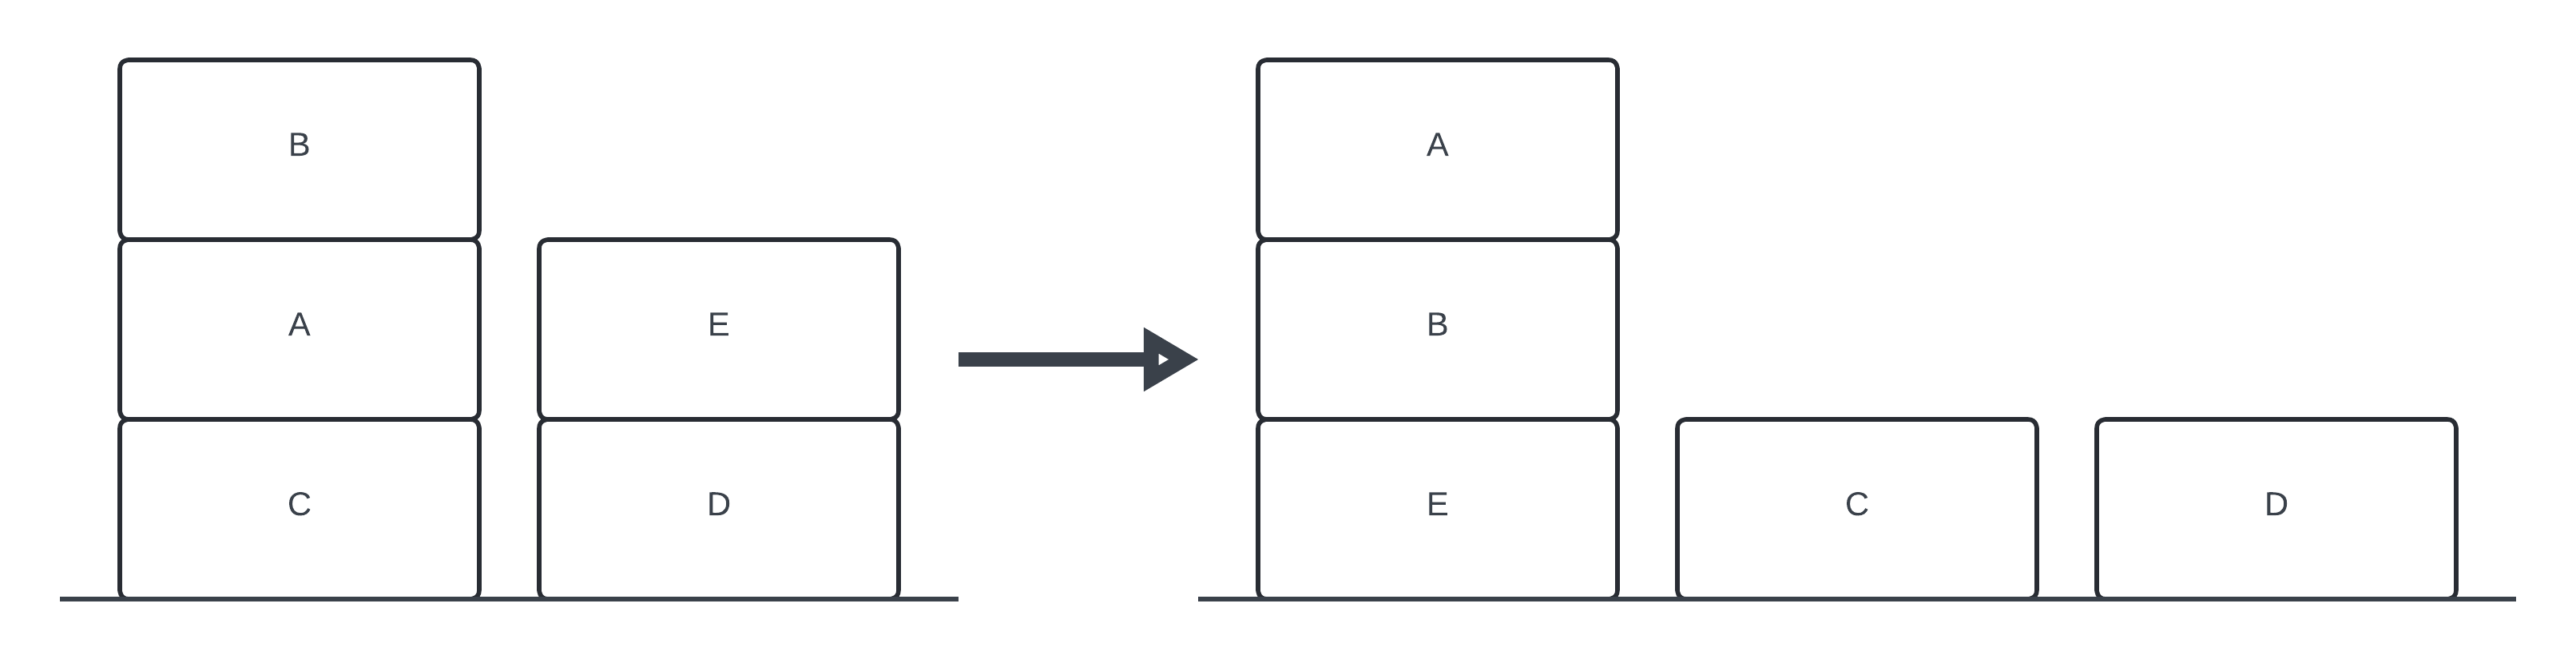
\includegraphics[width=1\linewidth]{figures/blocksworld_visualized.png}
    \caption{\textit{Una visualizzazione del problema considerato per il dominio blocksworld}}
\end{figure}
\paragraph{Soluzione}
\begin{figure}
    \centering
    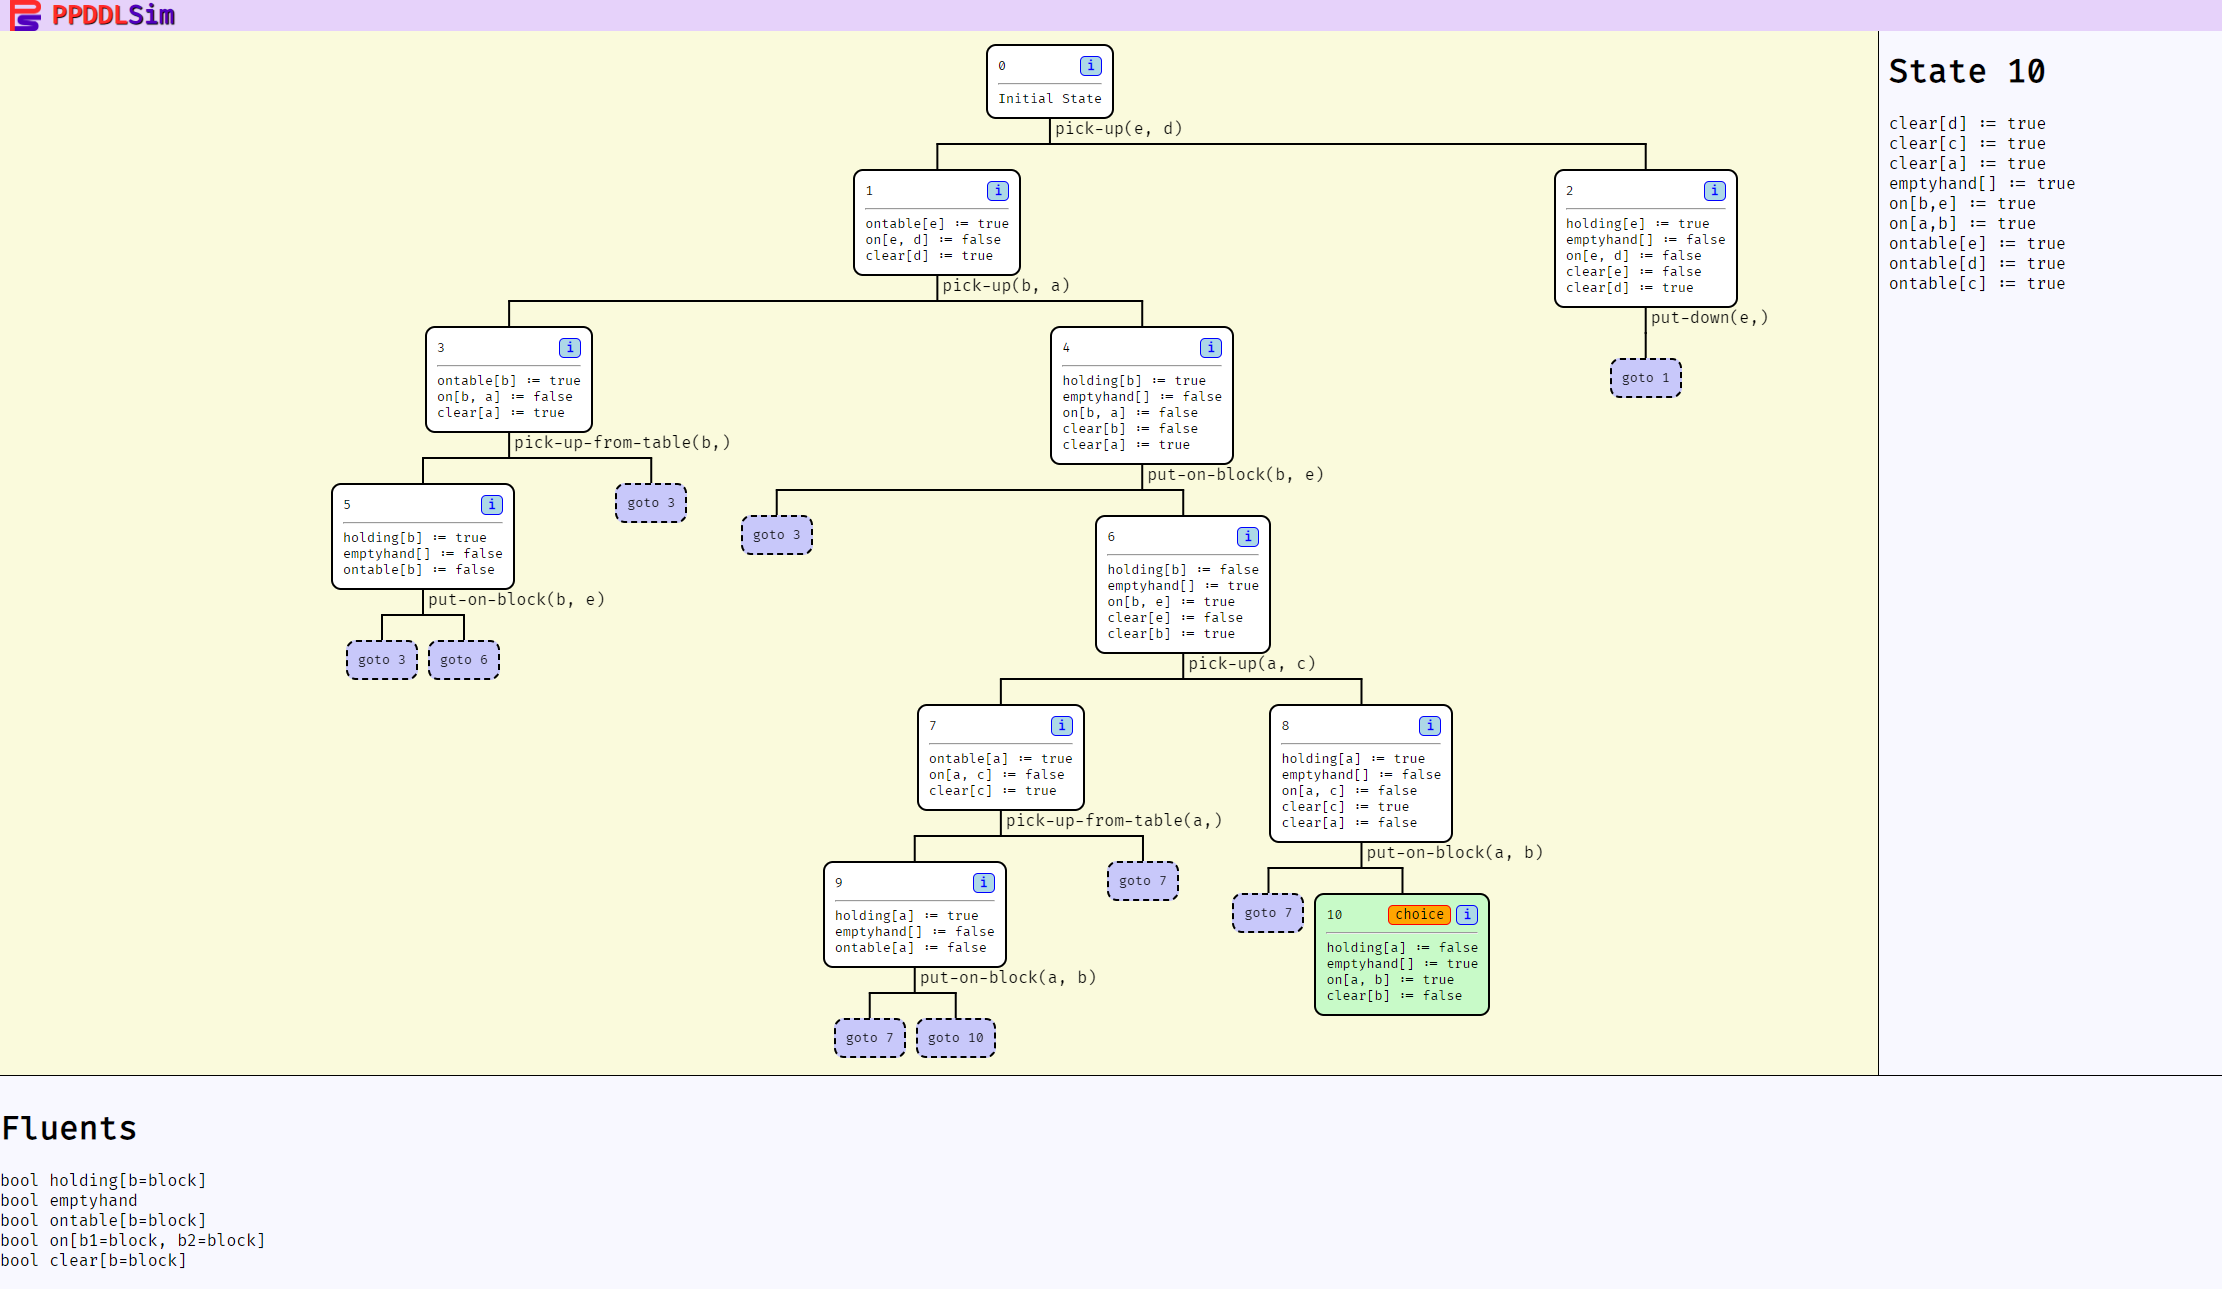
\includegraphics[width=1\linewidth]{figures/blocksworld_solved.png}
    \caption{\textit{Una soluzione del problema considerato per il dominio blocksworld}}
    \label{fig:soluzione}
\end{figure}
In \textit{fig. \ref{fig:soluzione}} è mostrata una soluzione al problema. Possiamo vedere che è una soluzione valida dal fatto che l'albero non ha foglie (all'infuori dello stato 10 che è finale e dei vari $goto_n$) e non ha loop. Questa soluzione consiste nel muovere il blocco $E$ sul tavolo, $B$ su $E$ e in fine $A$ su $B$. \\
Nel caso in cui ogni una di queste azioni fallisca si tenta di rimediare prima di muoversi al passaggio successivo. 

\chapter{Conclusioni e lavori futuri}
In questa tesi ho presentato i requisiti e una prima implementazione di un simulatore capace di gestire azioni non deterministiche nel contesto dei domini PDDL. L'obiettivo primario è stato quello di dimostrare le capacità e le potenzialità di un simulatore di questo tipo.

I risultati ottenuti mostrano che il simulatore è in grado di gestire un'ampia gamma di scenari non deterministici. Questo rappresenta un significativo passo avanti rispetto alle soluzioni precedenti e dimostra la validità dell'approccio adottato. Le performance del sistema, misurate in diversi contesti, hanno evidenziato una buona scalabilità e un tempo di esecuzione accettabile, anche per problemi di dimensioni medio-grandi.

Tuttavia l'implementazione corrente non supporta tutte le caratteristiche del linguaggio PPDDL, limitandosi solo alle azioni non deterministiche tramite clausole \texttt{oneof}. \\
Aggiungendo il supporto per le azioni probabilistiche si potrebbero illustrare le probabilità dei differenti outcome sugli archi del grafo, ma il funzionamento del simulatore non varierebbe.

Una versione futura del simulatore potrebbe includere la possibilità di esportare la simulazione svolta su un file. Questa prenderebbe la forma di una policy, che descrive gli stati e l'azione da compiere in ognuno di essi.

In sintesi, questa tesi ha fornito un contributo allo studio delle azioni non deterministiche nella pianificazione automatica, proponendo una soluzione pratica e implementabile per la simulazione di tali azioni. Sebbene il lavoro svolto abbia risposto alle principali domande di ricerca poste, rimangono aperte diverse possibilità di approfondimento, che potrebbero essere esplorate in futuri lavori.

\bibliographystyle{plainnat}
\bibliography{bibs/pddl,bibs/upf,bibs/flask,bibs/p5js,bibs/misc}
\end{document}

